\documentclass[letterpaper]{article}
\usepackage{natbib,alifeconf}
\usepackage{hyperref}

\title{Your Title: Something catchy that captures the main idea}
\author{Your Name\\
\mbox{}\\
Your PhD program, Indiana University\\
author@iu.edu}


\begin{document}
\maketitle

\begin{abstract}
{\bf What did you do in a nutshell?} An abstract summarizes, in one paragraph, the major aspects of the entire paper in the following prescribed sequence. First, the question(s) you investigated or purpose, from Introduction. State the purpose very clearly in the first or second sentence. Second, the experimental design and methods used, from Methods. Clearly express the basic design of the study. Name or briefly describe the basic methodology used without going into excessive detail -- be sure to indicate the key techniques used. Third, the major findings including key quantitative results, or trends from Results. Report those results which answer the questions you were asking, identify trends, relative change or differences, etc. Finally, a brief summary of your interpretations and conclusions. from Discussion. Clearly state the implications of the answers your results gave you. (Notice that given the content of the abstract, this is typically the last thing you have to write). Keep your abstract to about 200-300 words maximum.
\end{abstract}

\section{Introduction}



\section{Model and Methods}
{\bf How did you go about addressing the problem?} In this section, you should provide enough detail about your model and methods of analysis for anyone to be able to replicate precisely your results. Here's an example of an equation: 
\begin{equation}
    \tau_i \frac{dy_i}{dt} = -y_i + \sum_{i=1}^{N} w_{ji} \sigma(y_j+\theta_j) + I
\end{equation}
\noindent where $y_i$ represents the state of unit $i$ in the network, $\tau_i$ represents its time-constant, $\theta_i$ represents its bias, $w_{ji}$ represents the weight connecting unit $j$ to unit $i$, and $\sigma(x)$ represents a sigmoid function, in this case $\sigma(x)=1/1+e^{-x}$.

If your model is relatively complicated, you might want to consider also including a schematic illustration of the model (see Figure~\ref{fig1}). 

\begin{figure}[!htb]
\begin{center}

\includegraphics[width=2in]{fig1.png}
\caption{Model. The figure caption should give the reader enough detail to be able to look at the figure and read the caption and understand most of it. More detail is better than no details.}
\label{fig1}
\end{center}
\end{figure}

Keep in mind that, in principle, a reader should be able to skip the Model/Methods section and still make sense of what you accomplished. They may only return to the Model and Methods when they have technical questions about the details of how things were done.

\section{Results}
{\bf What did you find out?} In this section, you will tell us what experiments you ran, why you ran them, what results you observed, and how you have interpreted those results. If the results led you to ask more questions, then make sure to use that to motivate the next set of experiments. 

Do take some time to organize your results. Don't simply tell us everything you did in chronological order. You may consider re-ordering the experiments to facilitate the understanding of the narrative. 

When your paper reports on more than one experiment, use subheadings to help organize the presentation.

Also, importantly, make sure that you start each experiment with a motivating question. Avoid just telling us what you did, but start off telling us why you are wanting do learn something, and then tell us how you are going to go about answering that question. So, instead of: "Results paragraph: I ran a CTRNN 100 times and measured how well they oscillated. I observed this and that." Try something like this instead: "It is not well known whether a CTRNN can be trained to oscillate using local Hebbian learning rules without any global feedback. In order to begin to address this question, we set out to test how well the X learning rule (see Methods)  could allow the CTRNN to improve at task Y. We repeated the experiment 100 times to examine the reliability of the mechanism t." 

\begin{figure}[!htb]
\begin{center}
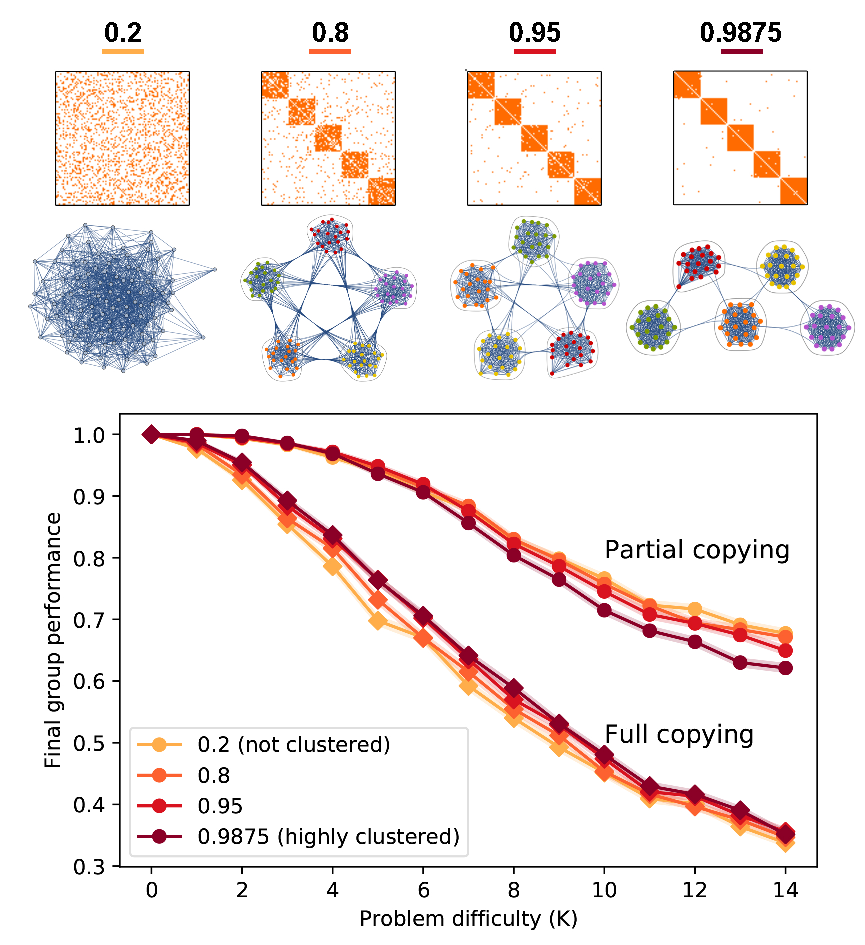
\includegraphics[width=\linewidth]{fig2.pdf}
\caption{Final performance across problem difficulty while varying groups across eight combinations on two dimensions: amount of clustering as determined by in-group probability (ranging from a random graph to a highly clustered graph) and copying (full or partial). Each point represents performance of the group of 100 individuals after 2,500 learning steps, averaged over 1,000 repetitions. Circles represent partial copying conditions; diamonds represent full copying conditions. Shaded area represents standard error around the mean. Above the plot is an example of an adjacency matrix and network visualization for each clustering condition. As the in-group probability increases, connections within communities visually become more dense while connections between communities become more sparse. The advantage of partial over full copying is robust regardless of the community structure.}
\label{fig2}
\end{center}
\end{figure}

When it comes to figures and captions. Make sure you take some time to polish your figure. Select colors appropriately and consistently. Make sure that the figure has all the appropriate labels and that the size of the fonts are legible. A reader should be able to see the figure and make sense of it. The caption should then help the reader understand all that is being shown in sufficient detail.

\section{Discussion and Conclusions}
{\bf  What does it mean?} Start off with a brief summary of the results and the main insights gained. Are there any things that came up during experiments and interpretation of the Results that warrant a further discussion. What are the limitations of your model. You are encouraged to be a good critic of the work and express honestly its shortcomings. End in a forward-looking note. What could be done next? What do you see as the most immediate next steps that you would do (or that somebody else reading your paper might want to set out to examine). 

{\bf How long should this document be?} It doesn't matter for now. If you end up with a two-page report, that's fine. If you end up with a longer one, that's fine too. Keep in mind that the point of this report is to efficiently communicate your scientific findings in a way that makes your claims supported by clear evidence, your methods reproducible, and your results easily interpretable. 

{\bf Additional reading?} Finally, take some time to do some additional reading on the structure of scientific papers. These are two resources that I think might be useful (they are both hyperlinks, so should should be able to click on them): 
\href{https://www.nature.com/scitable/topicpage/scientific-papers-13815490/}{"Scientific Papers by Nature"} and
\href{https://abacus.bates.edu/~ganderso/biology/resources/writing/HTWsections.html}{"The Structure, Format, Content, and Style of a  Journal-Style Scientific Paper"}. 

\footnotesize
\bibliographystyle{apalike}
\bibliography{bibliography}

\end{document}
